\subsection{The \HDEMO\ prototype}

\begin{figure}
  \begin{center}
    %\includegraphics[width=0.31\textwidth]{img/Fiber13D.png}
    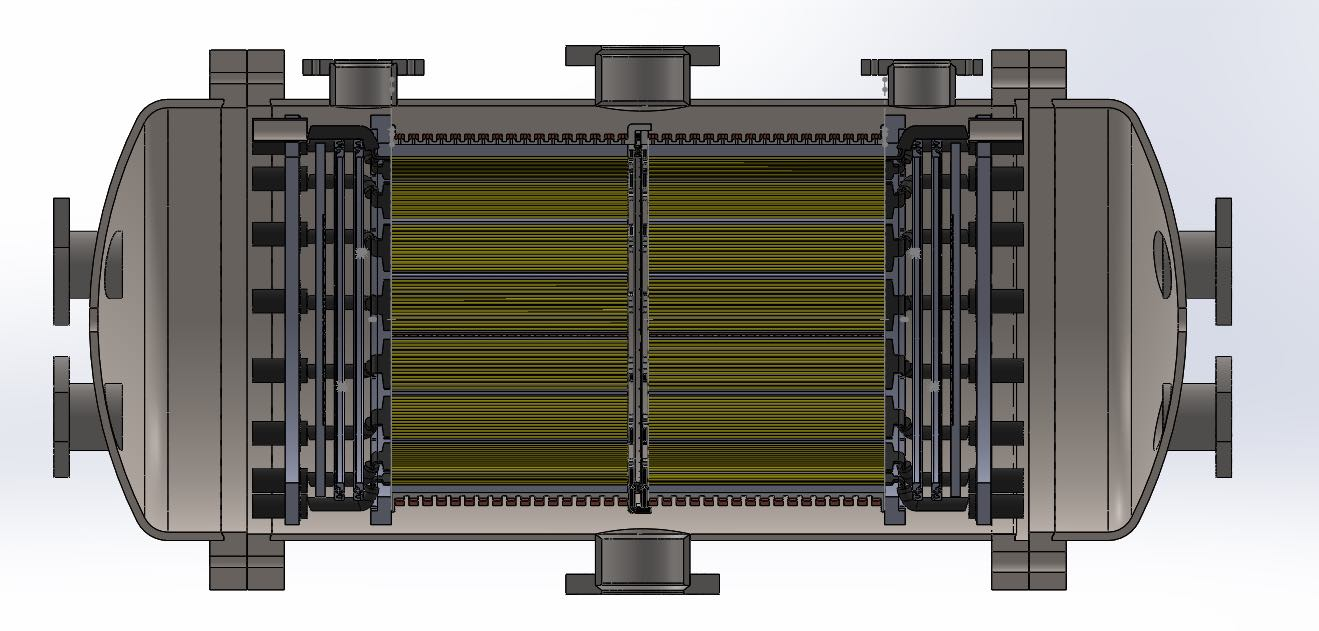
\includegraphics[width=0.61\textwidth]{img2/nhd_vessel.jpg}
    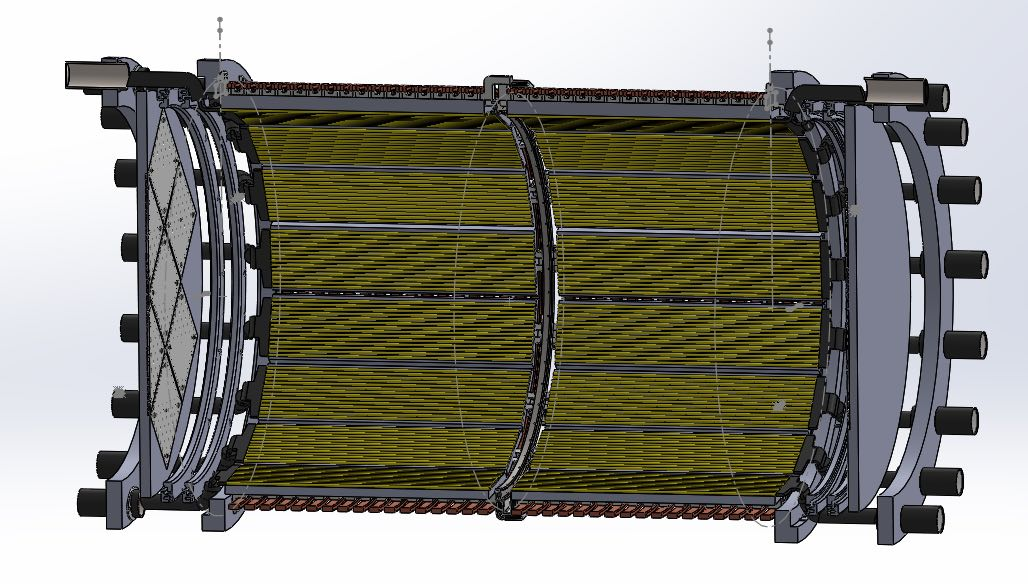
\includegraphics[width=0.55\textwidth]{img2/nhd_view.jpg}
    \caption{Conceptual design of the \HDEMO. The left panel shows a lateral view including the vessel. Notice the symmetric structure and the ports for
    the high voltage feedthroughs. In this design, shown in more detail in the right panel, the fibers are read out by PMTs disposed as a ring around the silicon planes.} 
    \label{fig.hdemo}
  \end{center}
\end{figure}


\indent


The R\&D towards \NHD\ requires the construction, commissioning and operation of a mid-size demonstrator that we call \HDEMO. The apparatus, shown in figure \ref{fig.hdemo}, will permit addressing several key questions. Specifically:

\indent


\begin{itemize}[noitemsep,topsep=0pt,parsep=0pt,partopsep=0pt]
\item Demonstrate the expected light yield and energy resolution of the BDF (we project 0.5\%--0.7\% FWHM). Decide whether the fibres will be readout using PMTs (as shown in figure \ref{fig.hdemo}) or by SiPMs. 
\item Demonstrate the improvement of the topological signature using DSPs and Xe-He mixtures. Find the best compromise between pitch, diffusion and cost. 
\item Assess the potential of new materials, in particular titanium vs low radioactivity steel alloys, for the pressure vessel and the grids. 
\item Gain experience with the construction and integration of a symmetric TPC (all previous NEXT incarnations have been asymmetric). 
\item Test the new electronics and DAQ for the BFD and DSP.
\item Develop the software to include the reconstruction of the BFD ---a new system, w.r.t. previous NEXT apparatus--- and to handle the higher density of DSPs (\eg, optimisation of the track deconvolution algorithms). Develop and test the Monte Carlo simulation of \HDEMO, as a test platform for the simulation of \NHD. 
\item Test the overall system integration. 
\end{itemize}

\indent


The detector will have a diameter of \HDD\ and a length of \HDL, divided in two identical halves. The central cathode will be at a high voltage of \HDHV, while the two anodes will be at ground. The vessel will stand a pressure in excess of 20 bars. The operational pressure will be the same than \Next\ (and foreseen for \NHD), \eg, 15 bars. The xenon mass at that pressure will be \HDM. 

\indent


The three main systems of \HDEMO\ are  prototypes of the three main systems of \NHD, namely the BFD ({\bf pBFD}), the DSPs ({\bf pDSP}) and  the TPC ({\bf pTPC}). The detector will be hosted in a pressure vessel ({\bf PV}) made of steel or titanium, and protected by an external lead shield, but no inner copper shield is necessary (the operation of the detector, with radioactive sources, does not require ultra-low background). The operation of \HDEMO\ requires a fully equipped laboratory and a state-of-the-art gas system, all of which will be provided by the laboratory hosting the apparatus (DIPC). 

\indent

The pBFD will be made of \pBFDNP$\times$2 panels of optical fibres. Each panel has \pBFDNFPP fibres, which are read out by \pBFDNSIPMPP\ SiPM
of size \pBFDNSIPM\ (main option) or by a PMT (alternative option). Prototype panels will be built at IFIC and Israel (see section on the objectives of \sIFIC).

\indent


The pitch of the DSPs will be chosen at the minimum practical size, \pDSP (one can later increase the effective pitch by software). The number of channels will be \pDSPC and the number of boards \pDSPB.  The boards will be constructed by Harvard, while UPV will be in charge of developing the FEE and DAQ, which will be prototypes of the electronics for \NHD (see section on the objectives of \sUPV).

\indent

Two symmetric TPCs will be built at DIPC. The R\&D for the TPC include finding ultra-radiopure resistors for the resistor chain, and comparing titanium and
steel grids in terms of stability and radiopurity. DIPC will also built the pressure vessel and the gas system. The detector will operate in a dedicated lab at DIPC (see section on the objectives of \sDIPC).

\indent

Reconstruction software, Monte Carlo simulation and calibration will play a very important role in the operation of \HDEMO. The reconstruction software must be modified to include the readout of the BFD, which differs substantially from the readout of the EP in \NEW\ and \Next. Calibration results are crucial to demonstrate the expected improved energy resolution and topological signature. The software and analysis of \HDEMO\ data will be lead by USC  (see section on the objectives of \sUSC).



